\documentclass{article}
\usepackage{amsmath}
\usepackage{amssymb}
\usepackage{hyperref}
\usepackage{graphicx}
\usepackage{xcolor}

\begin{document}

\begin{center}
    Bei Krankheit oder Verhinderung, Aufgaben per Mail:\\
    \textbf{peter.gierss@ihfg.uni-stuttgart.de}
\end{center}

\section*{Woche 1}
\subsection*{Aufgabe 1}
\begin{itemize}
    \item Reibungselektrizität: PVC Rohr mit Stoff \textcolor{gray}{(Elektronen werden abgestreift)}
    \item Elektrische Kraft: Kondensation
    \item Influenz: Induzierter Dipol
    \item Chemische Vorgänge: Elektrolyse
    \item Strahlung: Zerfall
    \item Ionisation
    \item Mechanisch trennen
\end{itemize}
\begin{equation*}
    \vec{F_C} = \frac{1}{4\pi\varepsilon_0}\cdot\frac{q_1q_2}{r^2}\hat{r} =\frac{1}{4\pi\varepsilon_0}\cdot\frac{q_1q_2}{r^3}r
\end{equation*}

\subsection*{Aufgabe 2}
\begin{center}
    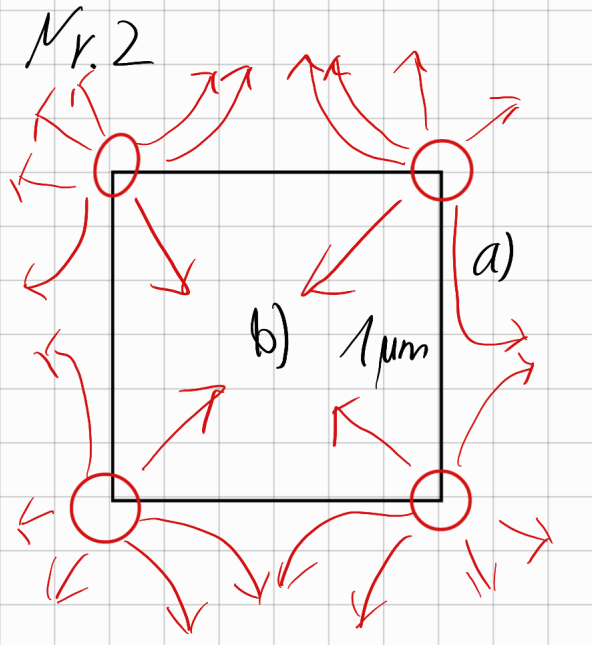
\includegraphics{Abbildungen/Abb.1.png}
\end{center}
\begin{itemize}
    \item[c)] Abstand der Protonen würde gleich bleiben, das ganze System bewegt sich mit.
\end{itemize}
\begin{equation*}
    \vec{F} = \frac{1}{4\pi \varepsilon_0}\cdot\frac{q_1q_2}{r^2} = 1151,94 \mathrm{\frac{V}{m}} 
\end{equation*}
Da:
\begin{equation*}
    \varepsilon_0 = 8,85 \cdot 10^{-12} \mathrm{\frac{As}{Vm}}
\end{equation*}
\begin{equation*}
    \cos(26,57) = \frac{A}{1151,94 \mathrm{\frac{V}{m}}} = 2060,57 \rightarrow \text{Durch 2} \rightarrow 1030,28 \mathrm{\frac{V}{m}}
\end{equation*}
\begin{equation*}
    \vec{F}=\frac{Q^2}{4\pi \varepsilon_0} \left[\frac{1}{a^3}\left(\begin{array}{c}0\\-a\end{array}\right)+\frac{1}{(a\sqrt{2})^3}\left(\begin{array}{c}-a\\-a\end{array}\right)+\frac{1}{a^3}\left(\begin{array}{c}-a\\0\end{array}\right)\right] = 4.42 \cdot 10^{-16} \text{ N } \cdot \frac{1}{\sqrt{2}}\left(\begin{array}{c}-1\\-1\end{array}\right)
\end{equation*}
\begin{equation*}
    \text{3 Proton} \rightarrow 2\vec{F}+\frac{1}{2}\vec{F}=5,75 \cdot 10^{-28} \text{ N}
\end{equation*}

\subsection*{Aufgabe 3}
\begin{center}paint
    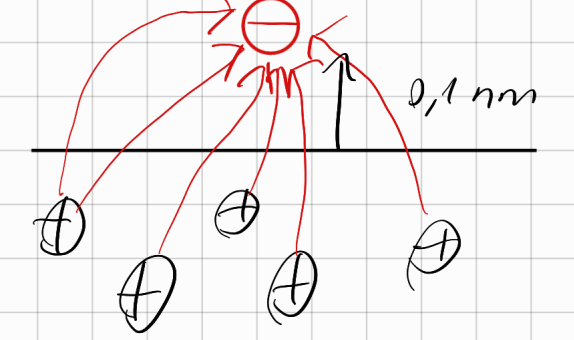
\includegraphics{Abbildungen/Abb.2.png}
\end{center}
\begin{equation*}
    w = \int \vec{F}\,d\vec{s}, \,F=\frac{Q_1Q_2}{4\pi\varepsilon_0}\frac{1}{(2x)^2}
\end{equation*}
\begin{equation*}
    w = \frac{Q_1Q_2}{4\pi\varepsilon_0} \int_{r}^{\infty} \frac{1}{(2x)^2}\,dx = \frac{Q_1Q_2}{4\pi\varepsilon_0} \left[\frac{1}{(2x)^2}\right]^\infty_r = \frac{Q_1Q_2}{4\pi\varepsilon_0} \cdot \frac{1}{4r} = 5.76 \cdot 10^{-19} \text{ J}
\end{equation*}

\subsection*{Aufgabe 4 (T)}
2-Achsiges Koordinatensystem, an den Achsen spiegeln, bis eine Punktsymmetrie zum Ursprung vom Ausgangspunkt entseht, bei einem spitzeren Winkel müssen mehr "Generationen" \textcolor{gray}{(Spiegelladungen)} auftreten, bis die Punktsymmetrie entsteht.

\subsection*{Aufgabe 5 (T)}
a) \begin{equation*}
    q_e = -1.6 \cdot 10^{-19} \text{ C}, \, r = 5.29\cdot 10^{-11}\text{ m} q_p = 1.6 \cdot 10^{-19} \text{ C}
\end{equation*}
\begin{equation*}
    F_{el} = \frac{1}{4\pi\varepsilon_0}\frac{|q_e|1_e}{r^2} = -8.2 \cdot 10^{-8} \text{ N}
\end{equation*}
b)
\begin{equation*}
    F_z = F_el
\end{equation*}
\begin{equation*}
    \frac{m_ev^2}{r}=\frac{1}{4\pi\varepsilon_0}\frac{|q_e|1_e}{r^2} \Rightarrow V = \pm \sqrt{\frac{1}{4\pi\varepsilon_0}\frac{|q_e|1_e}{r^2}} = 2.2 \cdot 10^6 \mathrm{\frac{m}{s}}
\end{equation*}
\begin{equation*}
    T = \frac{2\pi r}{v}=1.5 \cdot 10^{-16}\text{ s}
\end{equation*}
\end{document}